\documentclass[10pt]{article}
\usepackage{tmlr}
\usepackage{amsmath,amssymb,booktabs,graphicx}
\usepackage[hidelinks,pdfauthor={}]{hyperref}
\usepackage{url}

\title{Football Performance Dynamics Bench:\\ Information-Boundary-Aware Evaluation of Multi-Agent Football Motion}
\author{}
\hypersetup{pdftitle={Football Performance Dynamics Bench: Information-Boundary-Aware Evaluation of Multi-Agent Football Motion}}

\begin{document}
\maketitle

\begin{abstract}
A trajectory error is interpretable only when the information supplied to the model, the target representation, and the evaluated population are specified together. We present Football Performance Dynamics Bench, an evaluation framework developed by reconstructing a sequence of football performance and motion studies. The reconstruction records which scientific objects survive, which scores can be recomputed, and which results remain invalid, negative, or unrecoverable. We distinguish history-only forecasts from predictions conditioned on realized future ball or opponent trajectories, and separate target encoding from physical scoring and population standardization. Frozen task, measurement, evaluator, and result identities make these distinctions inspectable. We illustrate the framework using 18 frozen DeepSets checkpoints evaluated on four independent SkillCorner matches under a research-only descriptive protocol. The completed study binds 72 learned match-scoped records to common masks and 51,713 overlapping windows. In one shared-scope example, history-only displacement prediction yields average displacement error (ADE) of 1.6680 m, versus 2.2433 m for constant velocity. The example demonstrates the evaluation workflow for those matches and checkpoints. The original fit design remains incomplete and the protected population remains unqualified. Public artifacts permit contract execution and aggregate verification, while learned replay requires owner-private evidence.
\end{abstract}

\noindent\textbf{Keywords} \quad benchmark reconstruction, trajectory prediction, information boundaries, football tracking, reproducibility

\section{Introduction}

Two systems may each report three-second player-position error while answering different questions. One extrapolates what it can observe through the prediction origin. The other sees where the ball and opposing players will actually move. The second setting has legitimate uses in describing conditional motion, but its error has a different interpretation. Even with identical inputs, the same physical residual can produce different standardized errors after a change of reference frame. And adjacent origins share most of their observations, so the number of evaluated windows says little about the number of independent matches.

These distinctions matter when a benchmark is recovered from successive research studies. An evaluator can survive after its original inputs, calibration or fitted model have been lost. A measurement repair can preserve the task while changing which examples are evaluated. Treating the surviving artifacts as though they describe one uninterrupted experiment obscures what its results establish. We use Football Performance Dynamics Bench (FPD Bench) to examine how these distinctions can be made explicit in the evaluation itself.

We make three contributions. First, we reconstruct benchmark identities and result bindings from a mixed record of completed, invalidated, negative and unrecoverable work. The reconstruction yields different evidence classes for specifications, results and replay. Second, we formalize the information available at the prediction origin and pair that boundary with explicit target, evaluator and population definitions. This shows how physically equivalent residuals can receive different standardized scores and how membership rules can condition a history-only estimand. Third, we apply the contracts in a bounded four-match demonstration with frozen checkpoints, common truth masks, and match-first aggregation. An evidence chain connects the reported description to the research execution and identifies which links readers can check from public artifacts.

\section{Related work}

Conditional prediction has precedents in team sports. \citet{L1} model multi-agent sports sequences and generate trajectories given partial observations. \citet{L2} study soccer trajectory prediction, conditioning on other players' trajectories, and the competitiveness of linear extrapolation. \citet{L3} unify forecasting and completion in a trajectory model that represents predictive uncertainty. Our study concerns the evaluation question attached to each observed information regime. We use a simple set-based model and descriptive between-match variation. Predictive uncertainty and multimodal trajectory generation are outside our empirical scope.

Trajectory benchmarks already document target and evaluation choices. TrajNet++ evaluates interactions in pedestrian forecasting \citep{kothari2021}, while the nuScenes prediction benchmark specifies global-coordinate trajectories and best-of-$k$ displacement metrics \citep{nuscenesPrediction}. The latter is a different estimand from a single forecast with a fixed truth mask and equal-match aggregation. Our reconstruction examines how such choices affect comparability across successive versions of a benchmark and across conditional and ex-ante tasks.

The information boundary responds to a general leakage problem \citep{L4}. Declared access to realized future observations defines a conditional task. Undeclared access would invalidate a history-only interpretation. Blocked evaluation addresses dependence in structured data \citep{L5}; dataset-shift studies illustrate why the unit and population over which transfer is assessed need to be named \citep{L7,L10}. Here the physical match is the experimental unit. Repeated training seeds assess algorithmic variability, and deleting an evaluation match from the mean changes the descriptive summary without fitting a model. Cross-validation variance also cannot in general be recovered from fold dispersion alone \citep{L6}.

Datasheets and reproducibility guidance emphasize explaining dataset composition, use and the artifacts needed to check a claim \citep{L8,L9}. We apply that idea at the level of an individual result. A task contract can be publicly executable when the historical checkpoint or scored observations are unavailable. A digest can allow a reader to verify a recorded identity while leaving the bytes needed for a replay inaccessible.

\section{Historical reconstruction and benchmark identity}
\label{sec:history}

We began with the surviving research registry and result artifacts. We identified the sources for each reported task, then recorded its target, allowed inputs, temporal interpretation, reference frame and evaluation population. We traced results to the measurement state, split, evaluator configuration, model and output identity where those artifacts survived. We distinguished original records from later repairs and kept unknown fields explicit. Finally, we checked recovered mathematical behavior on public analytic and synthetic examples and checked metadata independently of historical inference. Figure~\ref{fig:genealogy} and Appendix~\ref{app:cards} summarize the reconstruction.

\begin{figure}[t]
\centering
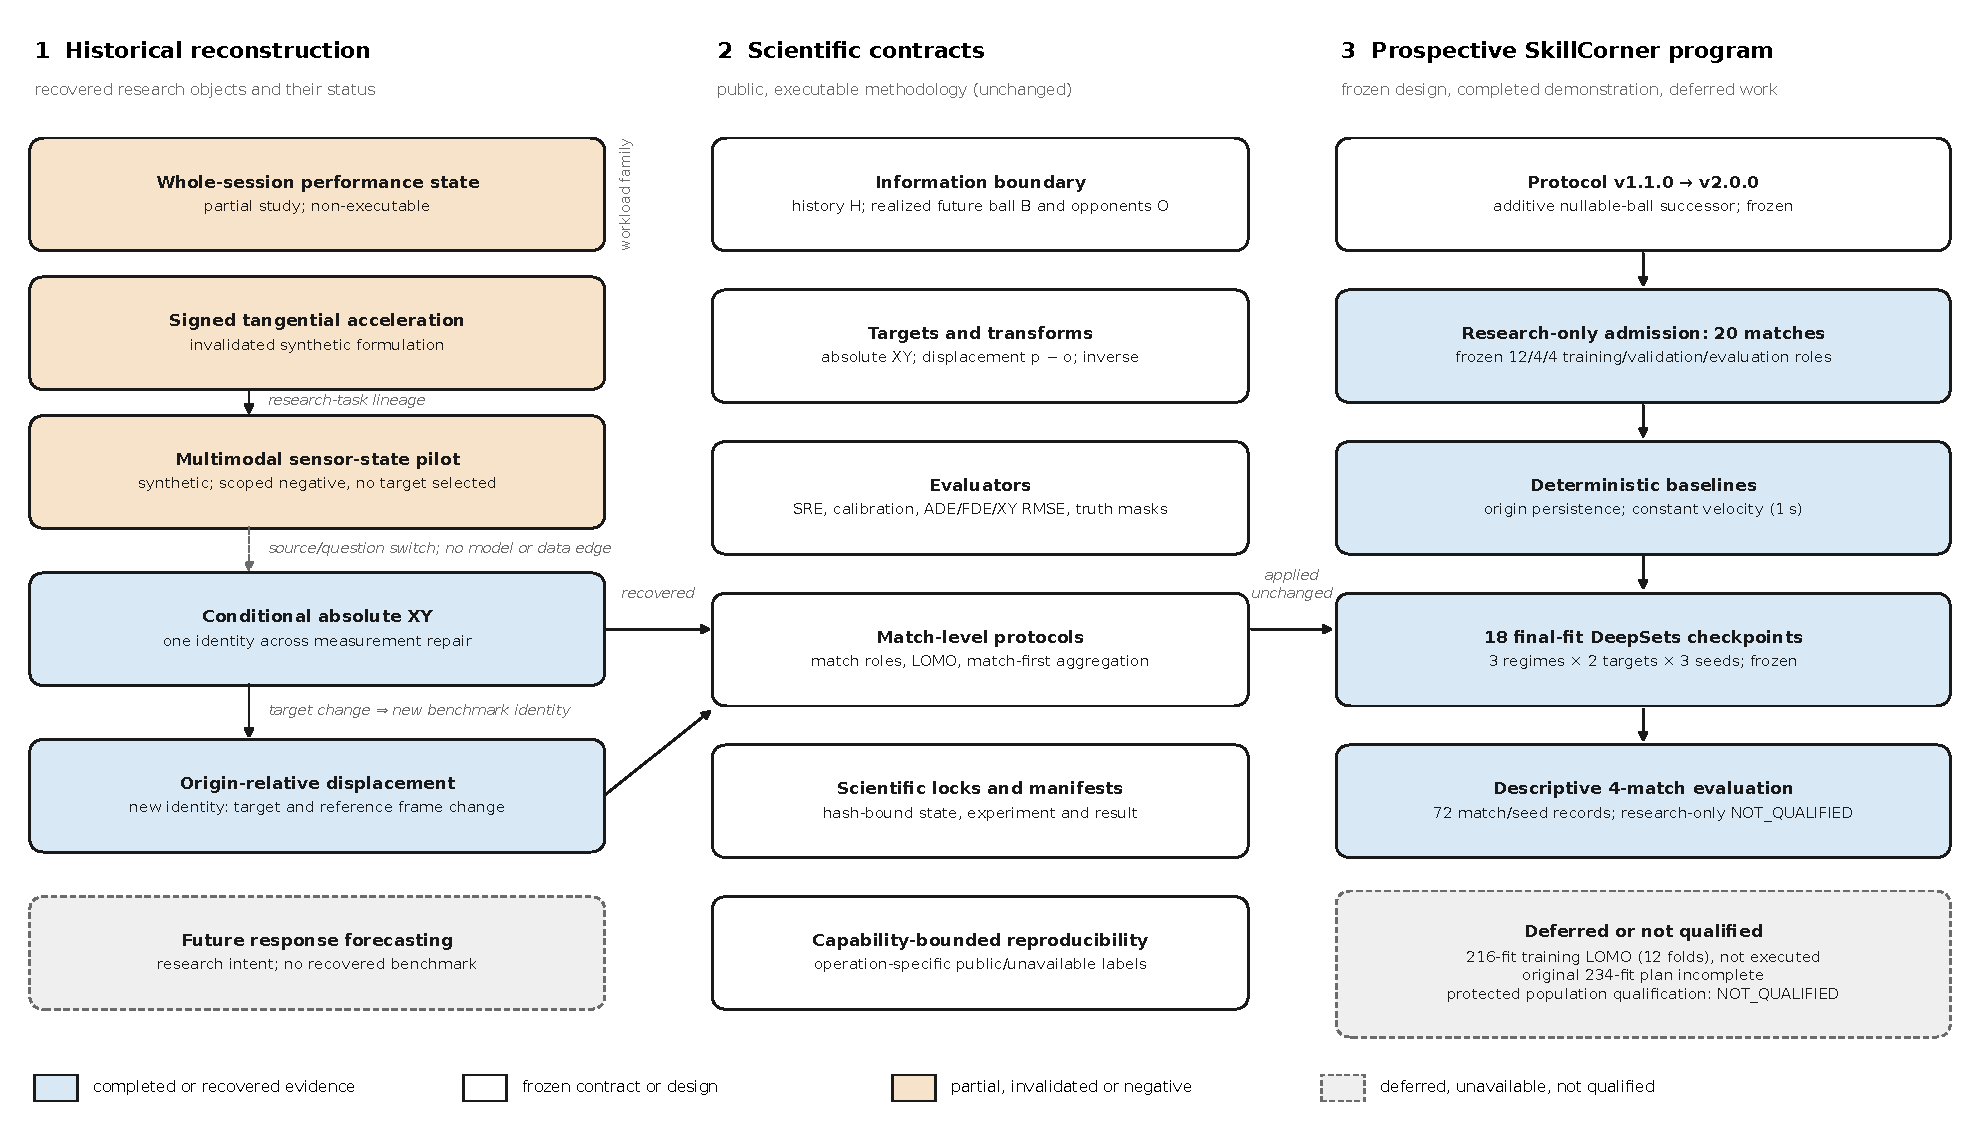
\includegraphics[width=\linewidth]{genealogy.pdf}
\caption{Reconstructed research families and the successor evaluation program. Arrows represent the indicated research or scientific transitions. Execution capability and evidential maturity are tracked separately. The SkillCorner study has its own source, measurements and task versions.}
\label{fig:genealogy}
\end{figure}

A research family groups questions. Its documented research objects can include partial studies, invalidated formulations, or a negative pilot without a viable benchmark. A benchmark specifies a scientific task. Source release, measurement state, dataset membership, split, evaluator, trained checkpoint, run and result each have their own identities. Scientific locks bind the applicable result-bearing state, whereas publication and hosting details belong to release metadata. Two scores with the same task identifier can still come from different populations or evaluator states.

The historical absolute-position task retained its identity through a measurement repair because its target, horizon and conditioning question were preserved. The repair changed eligibility, measurements, and surviving membership. The archived original study fell short of simple physical baselines, while later repaired-state match-held-out results met their own recorded viability gates. A row-level crosswalk between the populations was unrecoverable, so these results describe their respective scopes. The origin-relative redesign changed the target and reference frame, warranting a separate identity. Its originally reported aggregate was invalidated after a tuple-order assignment error. A later aggregation-only correction uses preserved fold outputs and checkpoint identifiers, without retraining. The generated displacement calibration was unrecoverable.

The other families illustrate distinct limits of recovery. The whole-session workload study lacks the specifications and result binding needed for standalone execution. A separate synthetic signed-acceleration formulation was invalidated, with its diagnostic metrics retained and its precise invalidation trigger unrecovered. A synthetic multimodal sensor-state pilot selected no target family within its recorded gate. Future response forecasting survives as research intent. These outcomes distinguish an evidence gap, an invalidated formulation, and a documented negative outcome.

\section{Information boundary}
\label{sec:information}

For a directed scene at origin $t$, let $H_t$ contain authorized observations through $t$, $B_t^+$ and $O_t^+$ denote realized ball and opponent trajectories at later samples, and $Y_t^+$ denote future target-team positions. Let $o$ be the observed target-player origins and $T$ the target transform. The input bundles and prediction are
\begin{equation}
 I_{\mathrm{history}}=H_t,\qquad
 I_{\mathrm{ball}}=(H_t,B_t^+),\qquad
 I_{\mathrm{full}}=(H_t,B_t^+,O_t^+),\qquad
 \widehat{y}=f_\theta(I_r),\quad y=T(Y_t^+,o).
\end{equation}
Only the history bundle is defined entirely by authorized observations through $t$. The other settings condition on events after $t$. They do not identify the effect of intervening on a player or ball trajectory.

\begin{figure}[t]
\centering
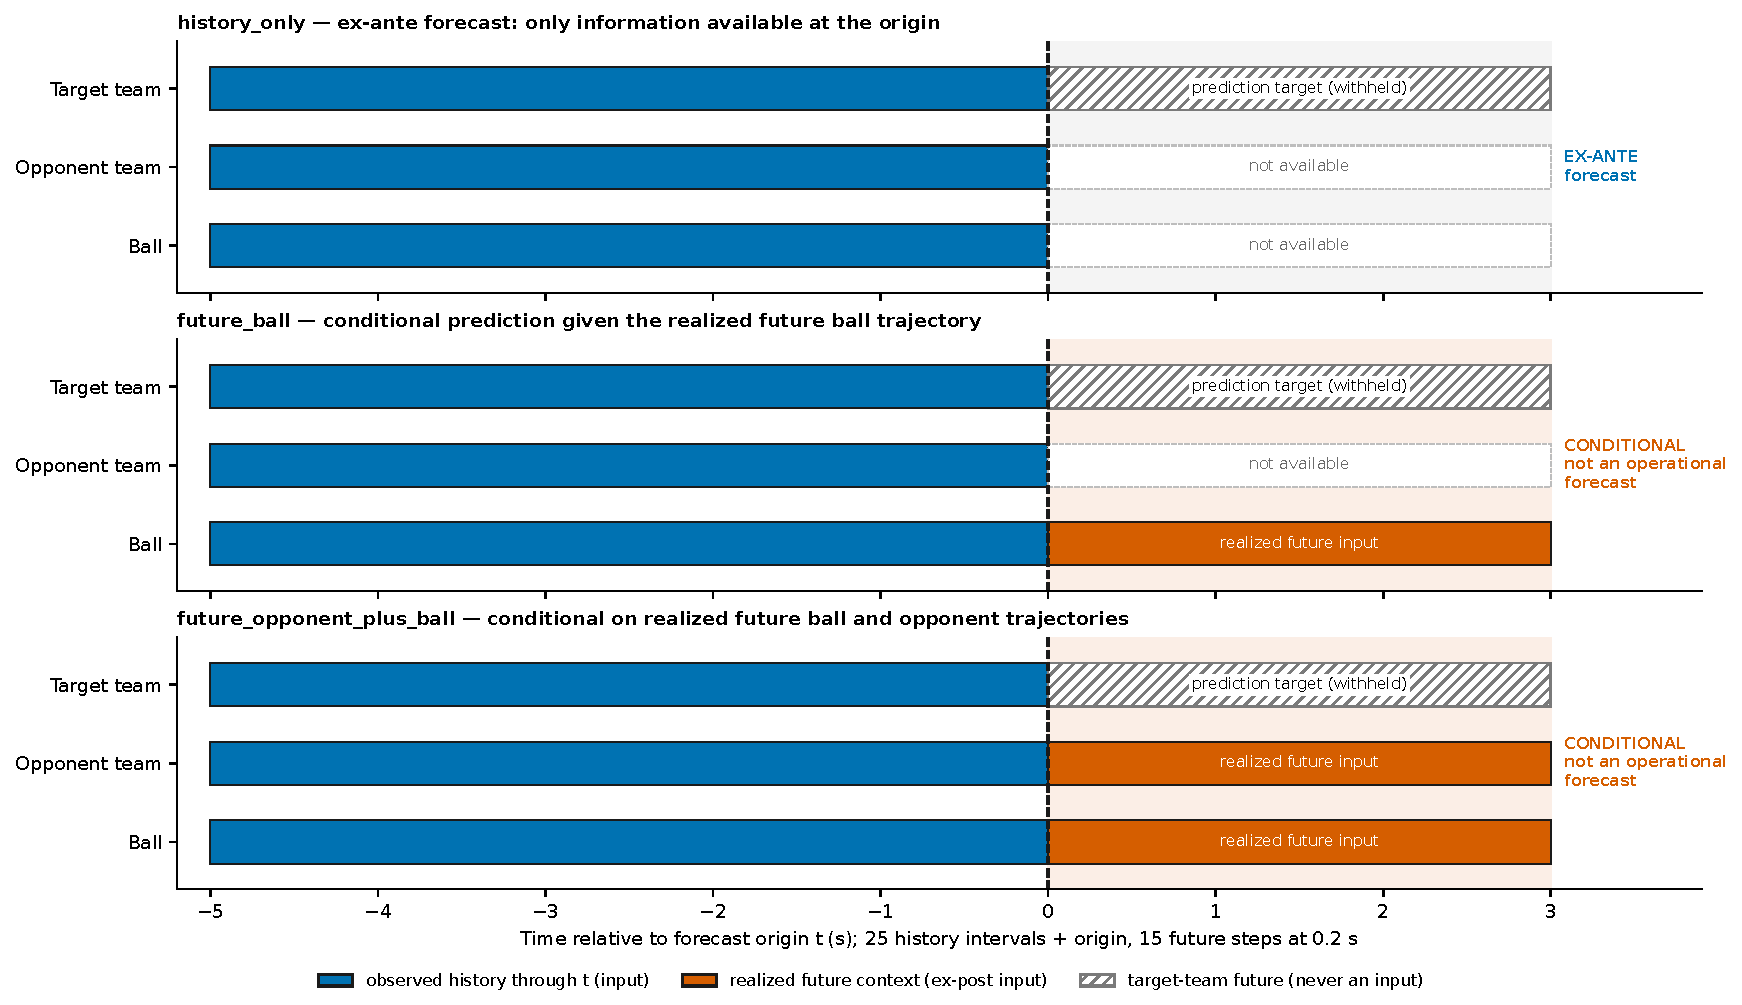
\includegraphics[width=\linewidth]{information-boundary.pdf}
\caption{Authorized inputs at the prediction origin for the three prospective regimes. History is shared. Future ball and opponent trajectories are supplied only in the named conditional regimes. Future target truth is reserved for scoring.}
\label{fig:boundary}
\end{figure}

The contract makes this boundary checkable (Figure~\ref{fig:boundary}). History times are finite, increasing and at or before the declared origin. The historical displacement contract also checks that the origin equals the final observed target frame. In the prospective task, history includes observed target, opponent and ball XY with presence masks, relative time and home/away side. Future conditional inputs have their own coordinates and presence masks. Provider identities align within-match records. Future target coordinates, target masks, future target membership, eligibility, phase and quality annotations, detection states, absolute clock, file identity, row order and numeric identity encodings are excluded from the learned features. The checks govern these channels and timestamp contracts. They cannot certify arbitrary upstream feature construction.

A membership rule may use future observations to decide whether a window is admissible. Under history-only scoring, this gives a forecast evaluated on a retrospectively defined eligible population. The model has no access to that eligibility decision as a feature. An operational evaluation would additionally have to define when to make a forecast and who is eligible without relying on future information.

\section{Targets, reference frames and evaluators}

\paragraph{Historical normalized targets.}
For future position $p$ and observed origin $o$, let $S=(52.5,34.0)$ m be the componentwise pitch scale. Historical targets use $a=p/S$ and $d=(p-o)/S$. Both arrays are $15\times11\times2$. The inverse of the displacement transform is $Sd+o$. When prediction and truth use the same origin,
\begin{equation}
 (S\widehat d+o)-(Sd+o)=S(\widehat d-d).
\end{equation}
Thus physical residuals are invariant to expressing the same prediction in the two frames. This says nothing about whether fitting a model in the two encodings produces the same prediction. The public synthetic check verifies the round trip to within $10^{-12}$ m.

\paragraph{Historical evaluator state.}
For each of the 330 scalar targets $j$, the historical raw evaluator computes $\mathrm{RMSE}_j$ over the declared evaluation population and divides it by the population standard deviation $\sigma_j$ of that target, with divisor $N$ in both moments. The historical binding uses $\mathrm{RMSE}_j$ when $\sigma_j=0$. The raw displacement score is the mean of these per-target standardized relative errors (SREs), with lower values preferred. Since origin subtraction can change the truth variance across rows, physical residual equivalence does not imply SRE equivalence. The historical absolute evaluator takes per-target SREs to clipped progress $\max(0,\min(1,1-\mathrm{SRE}_j/\min(f_j,c_j)))$ using frozen floors $f_j$ and ceilings $c_j$, then applies a locked piecewise-linear map to the equal-target mean progress. Its no-information, reference and perfect anchors are 0, 0.5 and 1. These are scoring anchors. They supply neither a displacement calibration nor measured validation performance.

\paragraph{Prospective metre-space metrics.}
The prospective task uses pitch-centered XY or $p-o$ in metres. It applies no pitch-scale normalization, rotation or attack-direction transform. The origin-player set is fixed through the horizon. Missing either future coordinate yields a null truth pair, without imputing a value or adding a replacement player. The model must furnish finite predictions at all required positions. For physical residual $e_{hi}$ at horizon step $h$ and origin player $i$, let $V$ be valid truth pairs and $V_H$ valid final pairs. Scene metrics are
\begin{align}
 \mathrm{ADE}&=|V|^{-1}\sum_{(h,i)\in V}\lVert e_{hi}\rVert_2,\quad
 \mathrm{FDE}=|V_H|^{-1}\sum_{i\in V_H}\lVert e_{Hi}\rVert_2,\\
 \mathrm{XY\text{-}RMSE}&=\sqrt{(2|V|)^{-1}\sum_{(h,i)\in V}(e_{hi,x}^2+e_{hi,y}^2)}.
\end{align}
If $V_H$ is empty, the scene has no score for any metric. If neither directed scene is scoreable, the window has no score. ADE is primary, FDE reports the final error, and XY-RMSE is a scalar-coordinate measure. The prospective evaluator has neither population SRE nor calibrated reward.

\section{Data, eligibility and experimental design}
\label{sec:design}

We use 20 matches from SkillCorner Open Data \citep{skillcorner}, a SkillCorner and PySport initiative, pinned at revision \nolinkurl{4340d274572876239c154c90bc507a9b3250a656}. The source contains provider-produced broadcast tracking. The historical reconstruction used a different source, with a 25 Hz input and a 5 Hz model grid. The prospective protocol selects source frames at 5 Hz from 10 Hz without interpolating target positions. Candidate origins advance by one retained sample within a period. A five-second history has 25 intervals and 26 samples including the origin. The three-second horizon contributes 15 samples.

Eligibility requires temporally continuous support, positive phase coverage over the underlying 10 Hz span, at least seven finite player positions per team at every support sample, a finite ball position at the origin and finite ball XY in at least 39 of the 41 slots. Phase annotations provide positive in-play evidence. An uncovered interval can also mean missing annotation. In version 2 ball-position availability and detection attribution are separate. The pinned-source rule for null detection with finite ball XY stops a qualification attempt rather than licensing silent filtering or a provider-wide interpretation of null. Source detection and quality annotations support diagnostics. Extrapolated player observations may still contribute scored physical targets.

\begin{figure}[t]
\centering
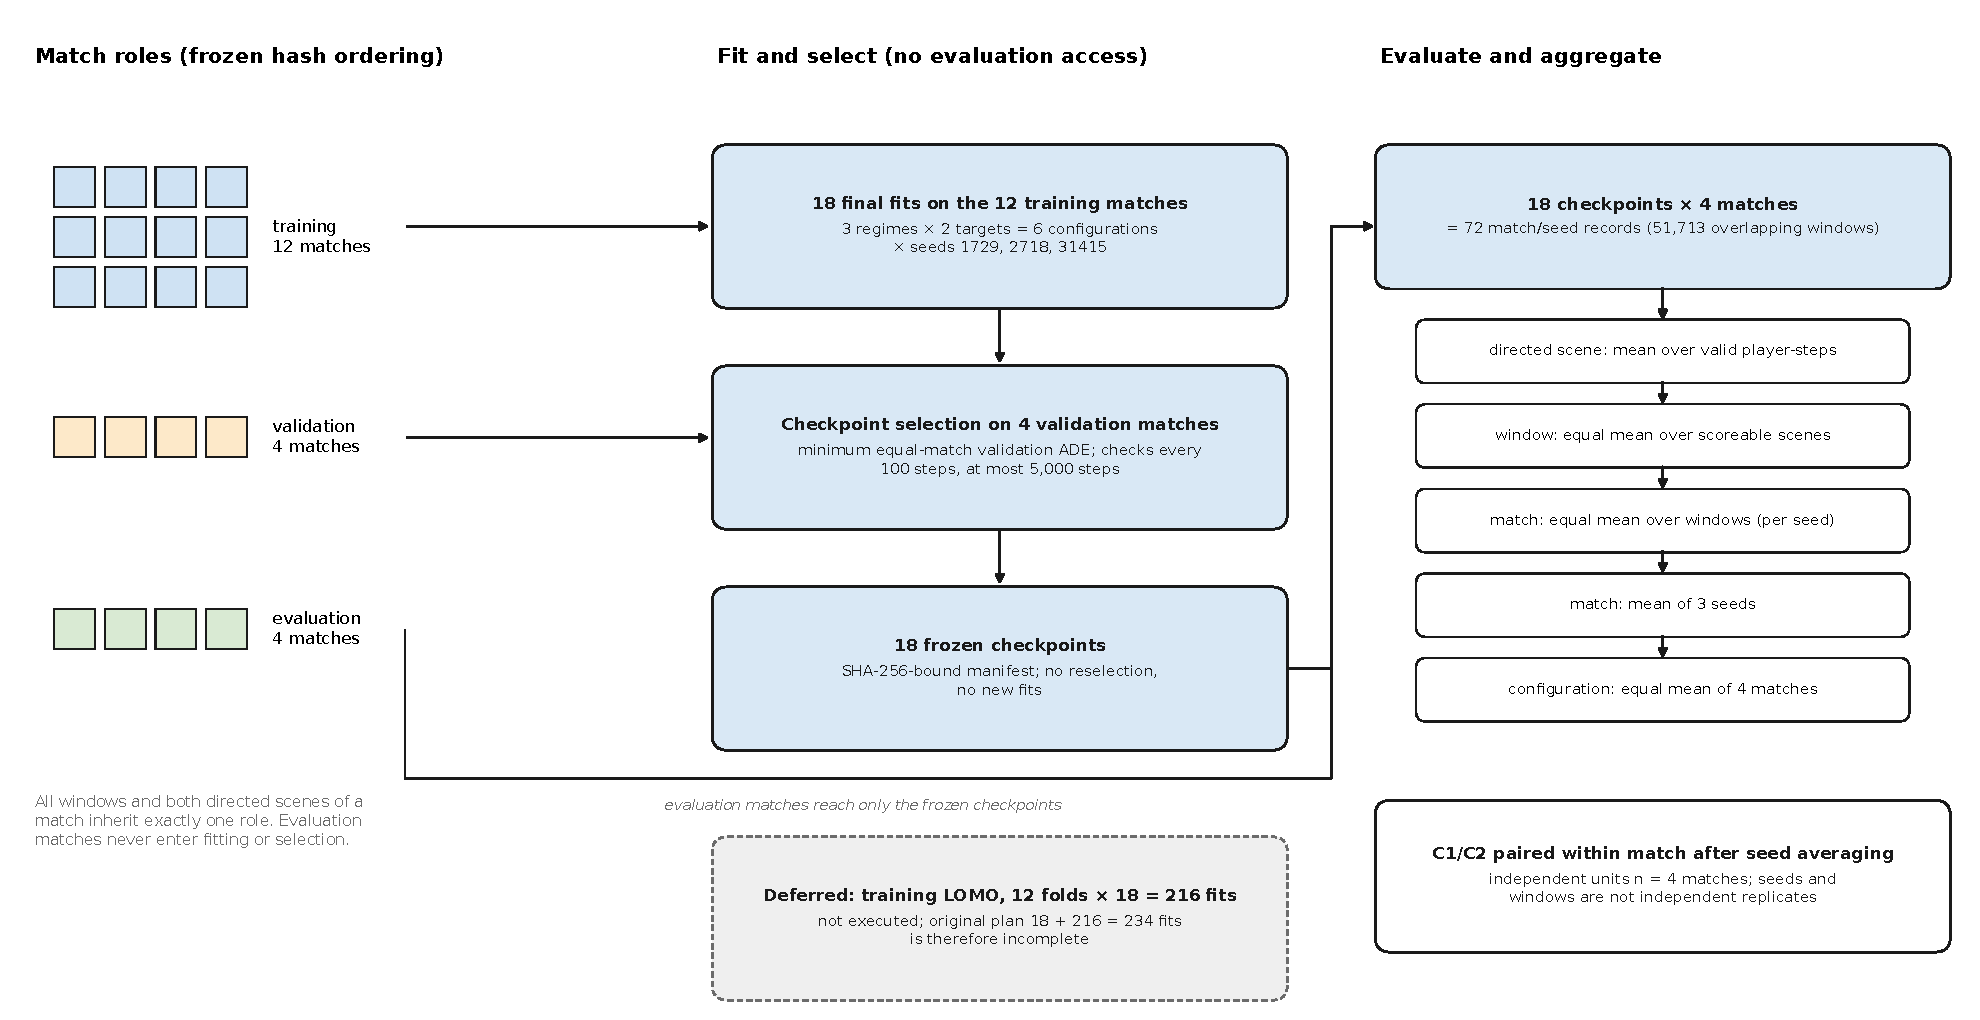
\includegraphics[width=\linewidth]{evaluation-design.pdf}
\caption{Match roles, checkpoint selection and aggregation. The two directed scenes inherit the physical window's match role. The frozen design and completed descriptive evaluation share the same roles and measurement endpoints.}
\label{fig:design}
\end{figure}

A frozen hash ordering of match IDs assigns 12 matches to training, four to validation and four to evaluation (Figure~\ref{fig:design}). The match is the experimental unit. Both directed scenes and all overlapping windows inherit its role. The 18 learned final fits cross two target encodings, three information regimes and three seeds for one per-target context DeepSets model \citep{zaheer2017}. The model encodes individual histories and pools team context with shared track encoders. Each checkpoint was selected on minimum equal-match validation ADE. The deterministic references are origin persistence and constant velocity estimated from a one-second causal history. Their physical predictions are invariant to target encoding. They use target history alone, whereas the learned history model sees broader scene history.

The original 234-fit design included 216 training leave-one-match-out fits across 12 training folds. All 216 remain deferred and unexecuted. A disclosed research-only amendment was frozen after validation and before observing any learned evaluation results. An initial learned scoring attempt terminated after entering scoring and left no committed, recovered or analyst-observed learned result. The four evaluation matches had already been used by deterministic controls. A distinct, separately authorized post-failure study evaluated the same frozen final checkpoints using the inherited endpoints and masks. The completed study is descriptive and the protected population remains \texttt{NOT\_QUALIFIED}.

For each metric, we average scoreable directed scenes equally within a physical window, and windows equally within match. For match $m$ and seed $s$, write the resulting score $q_{ms}$. The reported configuration summary is
\begin{equation}
 \bar q=\frac{1}{4}\sum_{m=1}^{4}\left(\frac{1}{3}\sum_{s=1}^{3} q_{ms}\right).
\end{equation}
Match size does not set its weight. Within-match seed variation describes repeated fits. Across-match variation describes the four observed matches. Neither the number of seeds nor the number of overlapping windows adds independent matches. The descriptive contrasts pair seed-averaged regime scores within match, subtracting future-ball ADE from history-only ADE, and full-context ADE from future-ball ADE, for each target encoding. Overall contrast directions cannot by themselves support a claim of improvement at every horizon.

\section{Reproducibility and evidence}

The result chain binds source release and population, canonical measurement, eligibility, task and split, evaluator, checkpoint, execution and result. The reconstructed historical scientific locks and the version 2 prospective authorities are separate. Each immutable result identity preserves the scope in which its values were computed. Display values may be rounded while the public aggregate representation retains full precision.

The completed learned study's authenticated readback checked a four-receipt chain, the required result inventory, source/checkpoint/code/runtime provenance, truth-mask denominator reconciliation and agreement with the independent metric audit. The archived analysis reconciled the reported summaries to the match-scoped records. This paper uses those recorded checks and published aggregates. Appendix~\ref{app:provenance} gives the identities and a public verification path. The distinction is material: synthetic checks verify specified behavior, public hashes allow consistency checks, and exact learned-result recomputation depends on owner-private inputs. None of these establishes independent protected-population qualification.

\section{Four-match demonstration}
\label{sec:demo}

The completed descriptive evaluation contains 18 frozen checkpoints, 72 verified learned match-scoped records and 51,713 overlapping windows from four independent evaluation matches. The record inventory corresponds to one score record per checkpoint and match. Counts and denominators agree with the frozen deterministic reference on the scored cohort. Both directed scenes were scoreable in each of the evaluated windows.

As a worked example, history-only origin-relative displacement achieved 1.6680 m ADE, compared with 2.2433 m for one-second constant velocity. Both scores refer to the same four matches, origin panels, physical truth masks and scoring hierarchy. The learned score uses seed averaging within match. The comparison concerns the fitted history-only system and its frozen kinematic reference, including their differences in available history. The pair illustrates how the reported units, scope and result binding can be checked before interpreting a numerical difference. It supplies no estimate of an isolated architecture effect.

\section{Discussion and limitations}

The reconstruction identifies three distinct failure modes for benchmark comparison. Measurement repair can change the evaluated sample under a stable task identity. Reference-frame changes can leave physical residuals intact yet change an SRE denominator. Future-derived eligibility can narrow a history-only evaluation even when a model sees no future features. In each case, an error value alone leaves the discrepancy unresolved. Maintaining separately bound task, population and evaluator records makes the comparison intelligible.

The demonstration uses a fixed cohort from one provider and one frozen model class. The four matches support a within-cohort description and do not establish statistical significance or generalization across leagues, teams, seasons or providers. Adjacent windows share observations. Much of the scored target data includes provider extrapolation, and agreement with provider tracking is distinct from agreement with independent ground truth. Scored windows need not represent excluded phases or difficult-to-observe players. The conditional regimes provide realized context and give no evidence about deployment with separately forecast ball or opponent trajectories. The study does not identify causal or tactical mechanisms.

Future studies could test transfer using additional rights-cleared matches and providers, assess measurement error against independent observations, and specify ex-ante policies for forecast issuance. They could also compare realized-context conditioning with predictions supplied by an upstream forecasting system whose errors are measured. Each would require a separately scoped evaluation. The deferred training folds and the unrecovered artifacts supply no results for those questions.

\section{Conclusion}

A football motion score depends on which observations were available at the origin, which players and windows were scored, and how their errors were aggregated. FPD Bench makes these choices explicit in the benchmark identity and the result's evidence chain. The historical reconstruction preserves negative and invalidated outcomes alongside executable contracts. The four-match demonstration shows how the same framework binds a bounded empirical result to its information regime, population, physical metric and provenance.

\section*{Data and code availability}

SkillCorner Open Data is acquired from the provider at the stated revision. The package contains source references, non-reconstructive schematics and an aggregate demonstration. It does not redistribute provider rows or row-level derivatives. Project code is available under Apache~2.0. The appendix describes public checks, with the identifying repository link omitted in the anonymous copy. Historical full fixture regeneration and learned inference lack public artifacts. The completed learned evaluation's checkpoints, match/seed input bundle, receipt bodies, private ledger, truth masks and predictions are owner-private. They are outside the public reproducibility claim.

\section*{Ethics and broader impact}

The study uses existing broadcast-derived football tracking and reports aggregate errors. Individual-level trajectories and identifiers are withheld from the publication package. Public access to source material does not establish redistribution rights for derivatives or weights. Motion estimates could be overinterpreted in consequential player assessment, especially where tracker coverage varies. To limit that risk, the evaluation reports the provider measurement scope, restrictions on inputs and population, and the distinction between descriptive errors and evidence appropriate for operational decisions.

\bibliographystyle{tmlr}
\bibliography{references}

\clearpage
\appendix
\section{Benchmark cards and reconstruction evidence}
\label{app:cards}

\paragraph{Historical conditional absolute position.}
The directed scene contains 11 target players, 11 opponents and a ball. Fixed arrays contain 25 history samples and 15 future samples on the 5 Hz model grid. The conditioning fields contain realized future opponent and ball trajectories. The target is normalized pitch XY. The public evaluator exposes population-standardized relative error (SRE), an absolute-position calibration, and separately bound physical diagnostics. Original and repaired measurements have distinct memberships, with no recovered row-level crosswalk.

\paragraph{Historical conditional displacement.}
The task retains the fixed-array conditional setting and substitutes normalized offsets from each player's observed origin. The displacement inverse and raw population SRE are executable. The generated displacement calibration and complete historical training/selection parity are unavailable. The corrected aggregation combines preserved fold results. The originally reported displacement aggregate is invalid.

\paragraph{Version 2 SkillCorner tasks.}
Both target encodings use 26 history samples including the origin, 15 future samples, and a variable panel selected from finite-XY origin players. History, history plus realized future ball, and history plus realized future ball and opponents define the three information regimes. A future missing target coordinate invalidates that XY pair. A scoreable directed scene needs a valid final pair. Physical metrics evaluate the same windows, panels and truth masks across configurations. Intended use is research on this specific admissible population. Protected-population status is \texttt{NOT\_QUALIFIED}.

\paragraph{Other historical research objects.}
The whole-session workload study is unrecoverable as an executable experiment. The synthetic signed tangential acceleration formulation is invalidated, and its exact invalidation trigger remains unknown. The native-rate synthetic sensor pilot selected no candidate target within its gate. Future response forecasting has no recovered target, population or scorer. These records constrain the genealogy in Figure~\ref{fig:genealogy}.

\section{Source, protocol and result provenance}
\label{app:provenance}

The study uses the pinned SkillCorner public source revision given in Section~\ref{sec:design}. The source authority specifies the match inventory, upstream paths and source checksums. The measurement and eligibility authorities specify the 10-to-5 Hz mapping and distinguish positional presence, detection attribution and missing support. Data acquisition is from the provider. The four evaluation matches are 1874553, 1925299, 2006229 and 2010085, with 12,363, 14,018, 12,501 and 12,831 eligible windows respectively. Each eligible window contributes two directed scenes in the completed study. Their counts apply to the common evaluated population for the 18 cells.

\begin{table}[h]
\centering
\caption{Protocol and result identifiers. The first two values are scientific-state digests. The remaining values are file digests.}
\label{tab:digests}
\begin{tabular}{@{}ll@{}}
\toprule
Authority & SHA-256 \\
\midrule
Prospective protocol v2 & \texttt{\scriptsize 3d7bdc46300b966a4da274579d21ac4c8219e1ef897719d6b7a308596e9f1d9f} \\
Original experiment plan v2 & \texttt{\scriptsize a59fee6ee8e9fb03f4f0ccdae1933458af2bbf2375db7e6cd2bdf10962e42b62} \\
Frozen checkpoint manifest & \texttt{\scriptsize 770f1d9bbca3020237992181a56e4f5be4adaae7aab07f5f1313aa699d8693e0} \\
Post-failure descriptive protocol & \texttt{\scriptsize ac931391ecb0afcb68974e1765f65fbff17071ade2bcaab93bdadd22f84a0305} \\
Frozen deterministic reference & \texttt{\scriptsize 21b19a2370d5b4a45652a6ce132cb3e78a4abe2027a096a71f383b1191ea9b36} \\
Completed private result file & \texttt{\scriptsize 82c8b31c5146523415430261936045ce4855a475dd4bbd874a4c01211d4cb6dc} \\
\bottomrule
\end{tabular}
\end{table}

The post-validation amendment bound the 18 already fitted checkpoints before learned evaluation results were observed. The first attempt entered scoring and yielded no committed, recovered or analyst-observed learned result. The completed descriptive study used a distinct execution scope. Its authenticated readback checked the four sealed receipts, source/checkpoint/code/runtime provenance, the ordered record inventory, denominators and independent metric-audit agreement. Aggregates were reconciled to the bound records without replay. Deterministic evaluation controls predate the completed execution.

\section{Reproduction capabilities and evidence index}

The public Python 3.12 checkout contains executable synthetic and analytic checks. These exercise target and information contracts, evaluator behavior, and the hashing and metadata chain. From a copy of that checkout, run the following with \texttt{uv}. The commands use tracked public artifacts and do not run the learned campaign.

\begin{verbatim}
uv sync --locked --all-groups
uv run --locked fpdbench validate
uv run --locked fpdbench evidence validate
uv run --locked fpdbench reproducibility check
uv run --locked fpdbench data-states verify skillcorner_5hz_v2
uv run --locked fpdbench eligibility verify skillcorner_window_v2
uv run --locked pytest -q tests/unit/test_benchmark_contracts.py
uv run --locked pytest -q tests/unit/test_prospective_trajectory_metrics.py
uv run --locked pytest -q tests/unit/test_paper_a_evidence.py
uv run --locked pytest -q tests/unit/test_res440_analysis.py
\end{verbatim}

\begin{table}[h]
\centering
\caption{Evidence supporting the paper's main claims.}
\label{tab:evidence}
\begin{tabular}{@{}p{0.28\linewidth}p{0.67\linewidth}@{}}
\toprule
Claim & Evidence and check \\
\midrule
Task identity and historical scope & Research-object registry, transition graph, archived result bindings and validity decisions. Public validation checks the contracts and reference inventory. \\
Boundary and target semantics & Frozen protocol, forecast-origin, feature-boundary and target contracts. Synthetic cases exercise rejected fields, origin inversion and metric denominators. \\
Scoring and match-first aggregation & Physical evaluator and mask tests, study protocol, published aggregate records and deterministic reference. Section~\ref{sec:demo} reports the shared-scope example. \\
Study provenance and availability & Table~\ref{tab:digests}, public aggregate account and authenticated readback. Public checks establish identity and consistency of the published metadata. \\
\bottomrule
\end{tabular}
\end{table}

The public package permits verification of recorded identities, counts and aggregate results. Strict resolution of historical evidence requires the canonical local registry. Recomputing learned aggregates from individual match/seed records requires the owner-private result bundle. Checkpoint bytes, receipt bodies, private ledger material, truth masks and individual predictions are withheld. Historical private qualification truth is forbidden and historical full fixture/inference replay is unavailable. Source rows and row-level derivatives remain outside the release, as do weights pending rights clearance. The empirical report is limited to the completed descriptive execution. The planned 216 training LOMO fits were unexecuted.


\end{document}
